\documentclass[11pt]{article}
\usepackage[a4paper,margin=2.2cm]{geometry}
\usepackage{amsmath}
\usepackage{booktabs}
\usepackage{graphicx}
\usepackage{array}
\usepackage{xcolor}
\usepackage[colorlinks=true,urlcolor=blue]{hyperref}
\usepackage{parskip}
\graphicspath{{figures/}}

\title{\vspace{-1.5em}HW2 - Kafka/Redpanda Throughput Investigation\\[0.3em]
\large Distributed video-frame pipeline}
\author{UCU - Data Streaming / Kafka}
\date{\today}

\begin{document}
\maketitle
\vspace{-1.5em}

\section{Overview}

A dummy distributed application in which microservices communicate through a
3-broker \textbf{Redpanda} cluster. A \emph{generator} splits a $\sim$30-minute video into
frames and publishes them; a pool of \emph{consumers} (one Kafka consumer group)
imitates processing by sleeping 1\,s per frame and logs a timestamped CSV row per
frame; an \emph{aggregator} computes system throughput and end-to-end latency. We
sweep the number of producers, partitions and consumers and measure the effect.

\textbf{Dataset.} ffmpeg generates a synthetic 30-minute test video, from which 200
evenly-spaced JPEG frames are extracted ($\approx$22\,KB each, 4.55\,MB total). Each
frame is one Kafka message.

\textbf{Metrics.} With $\text{makespan}=\max(\text{finish\_ts})-\min(\text{send\_ts})$:
\[
\text{Throughput (Mbps)}=\frac{\text{total\_bytes}\times 8}{\text{makespan}\times 10^{6}},
\qquad
\text{Max latency (s)}=\max(\text{finish\_ts}-\text{send\_ts}).
\]
Replication factor is held at 3 across all experiments; only producers, consumers
and partitions vary.

\section{Experiment configurations}

\begin{center}
\begin{tabular}{clccc}
\toprule
\# & Configuration & Producers & Partitions & Consumers \\
\midrule
exp1 & 1p / 1part / 1c   & 1 & 1  & 1  \\
exp2 & 1p / 1part / 2c   & 1 & 1  & 2  \\
exp3 & 1p / 2part / 2c   & 1 & 2  & 2  \\
exp4 & 1p / 5part / 5c   & 1 & 5  & 5  \\
exp5 & 1p / 10part / 1c  & 1 & 10 & 1  \\
exp6 & 1p / 10part / 5c  & 1 & 10 & 5  \\
exp7 & 1p / 10part / 10c & 1 & 10 & 10 \\
exp8 & 2p / 10part / 10c & 2 & 10 & 10 \\
\bottomrule
\end{tabular}
\end{center}

\section{Results}

\begin{center}
\begin{tabular}{cl rrr c}
\toprule
\# & Configuration & Throughput & Max latency & Makespan & Active \\
   &               & (Mbps)     & (s)         & (s)      & consumers \\
\midrule
exp1 & 1p / 1part / 1c   & 0.18 & 201 & 200.9 & 1  \\
exp2 & 1p / 1part / 2c   & 0.18 & 201 & 200.9 & \textbf{1}  \\
exp3 & 1p / 2part / 2c   & 0.36 & 100 & 100.6 & 2  \\
exp4 & 1p / 5part / 5c   & 0.90 & 40  & 40.2  & 5  \\
exp5 & 1p / 10part / 1c  & 0.18 & 201 & 200.8 & \textbf{1}  \\
exp6 & 1p / 10part / 5c  & 0.90 & 40  & 40.2  & 5  \\
exp7 & 1p / 10part / 10c & 1.80 & 20  & 20.2  & 10 \\
exp8 & 2p / 10part / 10c & 1.79 & 20  & 20.3  & 10 \\
\bottomrule
\end{tabular}
\end{center}

\begin{figure}[h]
\centering
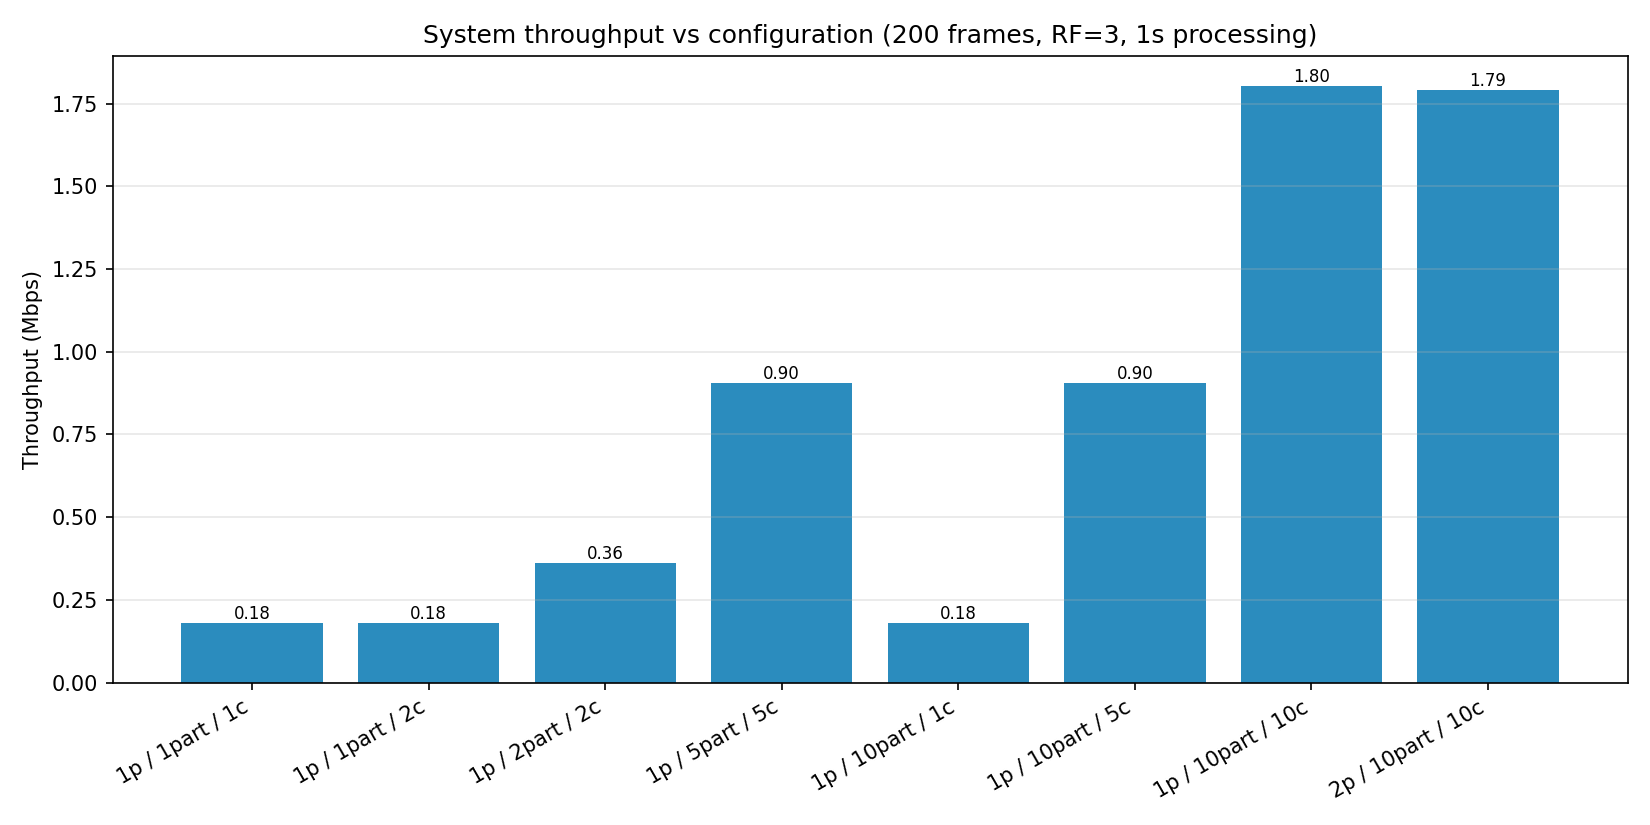
\includegraphics[width=\linewidth]{throughput.png}
\end{figure}

\begin{figure}[h]
\centering
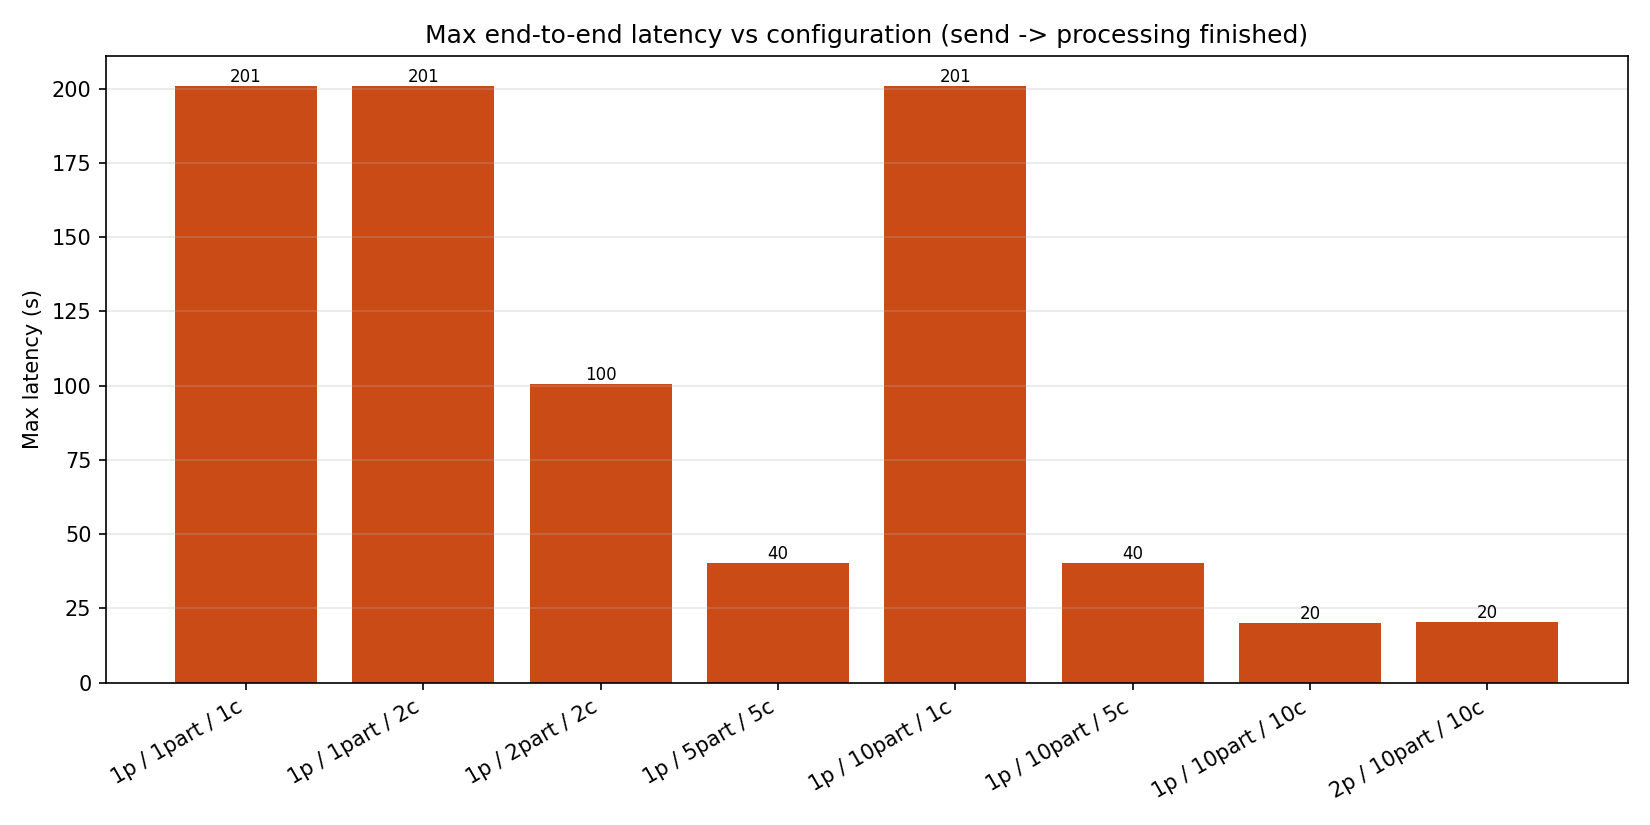
\includegraphics[width=\linewidth]{latency.png}
\end{figure}

\section{Findings}

\begin{itemize}
\item Throughput grows in proportion to the number of consumers that work at the
  same time, which equals $\min(\text{consumers},\text{partitions})$:
  $0.18\to0.36\to0.90\to1.80$\,Mbps for parallelism $1\to2\to5\to10$. Max latency
  goes down in the same proportion ($201\to100\to40\to20$\,s).
\item \textbf{exp2 $\approx$ exp1:} with one partition, the second consumer has no
  partition to read and stays idle (active consumers $=1$). The number of partitions
  sets how many consumers can work at the same time.
\item \textbf{exp5 $\approx$ exp1:} ten partitions do not help when there is only one
  consumer to read them.
\item \textbf{exp8 $\approx$ exp7:} a second producer does not increase throughput,
  because the speed is limited by the consumers (the 1\,s processing time), not by
  sending the messages.
\item The maximum throughput is set by the 1\,s sleep:
  $\text{parallelism}\times\text{frame size}\times 8 \approx 10\times22\text{KB}\times8
  \approx 1.8$\,Mbps, which matches exp7 and exp8.
\end{itemize}

\section{Deliverables}

\begin{enumerate}
\item \textbf{Source code:} \url{https://github.com/dchaplinsky/kafka-hw2}
\item \textbf{Run instructions:} see \texttt{README.md} (architecture, environment setup,
  and the exact commands for the cluster, dataset and experiment sweep).
\item \textbf{Graphs:} \texttt{figures/throughput.png}, \texttt{figures/latency.png}
  (reproduced above); raw numbers in \texttt{results/summary.csv}.
\end{enumerate}

\end{document}
